%!TEX root = ../draft.tex
\chapter{Theoretische Grundlagen}\label{s.grundlagen}
Das folgende Kapitel soll eine kurze und leicht verständliche Einführung sein, in der die theoretischen Grundlagen zu dem Aufbau von digitalen Bildern, dem Einfluss von Belichtung sowie den verwendeten Bildbearbeitungsmethoden gelegt werden. Anschließend folgt ein Überblick über die Grundlagen der künstlichen Intelligenz. Der letzte Abschnitt widmet sich den Schwerpunkten der künstlichen neuronalen Netze. Dabei werden hauptsächlich für die Arbeit relevante Grundlagen vermittelt. 
\section{Digitale Bilder}\label{s.digibilder}
Damit der Ansatz der These dieser Arbeit nachvollziehbar wird, soll in diesem Abschnitt auf die Aufnahme digitaler Bilder mit deren Eigenschaften und Aufbau eingegangen werden. Außerdem sollen die Schwächen herausgearbeitet und mögliche Lösungsansätze erläutert werden. Zunächst folgt eine kurze Einführung.\\\\
Bildverarbeitung wird in der heutigen Zeit oft mit Bildbearbeitung assoziiert, also mit der Bearbeitung von Bildern mittels Bearbeitungssoftware. In der Bildverarbeitung geht es, anders als in der Bearbeitung, um die Software selber, welche für die Konzeption und Erstellung von digitalen Bildern genutzt wird. Die digitale Repräsentation eines aufgenommenen Bildes erfolgt als zweidimensionale Matrix, wie in Abbildung \ref{img:digitalesbild} zu erkennen, welche man nach Belieben lesen und verändern kann, um seine geplanten Ziele zu erreichen. Grundsätzlich bestehen digitale Bilder aus Rastern. Diese besitzen mehrere Werte, welche auch Pixel genannt werden. Die Werte entstehen je nach Menge der Farbabstufungen. Bei einem 8-Bit-Graustufenbild sind das normalerweise 256 Abstufungen. 
\begin{figure}
[h]
\centering
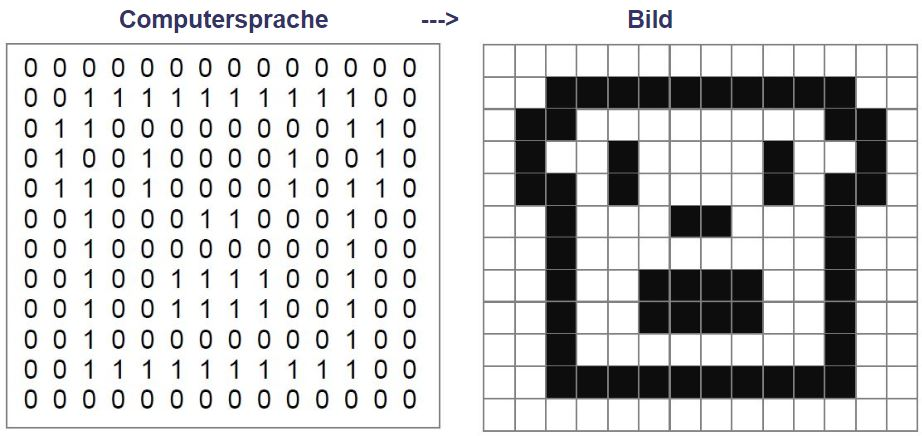
\includegraphics[scale=0.5]{Sources/Digitalesbild.JPG}
\caption{Aufbau eines Digitalen Bildes mit zwei Helligkeitsabstufungen}
\label{img:digitalesbild}
\end{figure}\\
In diesen Pixeln werden Bildinformationen, wie Farbe und Position festgehalten. Jeder Pixel besteht dabei oft aus drei Kanälen, dem R Kanal für Rot, dem G Kanal für Grün und dem B Kanal für Blau. Diese bilden in bestimmten Kombinationen und Intensitäten ungefähr 16 Millionen verschiedene Farben. Der beschriebene Aufbau wird bei RGB-Bildern verwendet und auch bei Monitoren, Smartphones, etc.. Neben dem RGB gibt es noch einige andere Farbräume \cite[309 ff.]{jahne2013digitale} (RGB, HSV, CMY(K), YUV, etc.).
\subsection{Farbräume digitaler Bilder}\label{s.aufbdigibilder}
Üblicherweise wird bei Digitalbildern mit dem RGB-Farbraum gearbeitet. Aus diesem Grund wird in dieser Arbeit hauptsächlich auf RGB-Bilder eingegangen. Ein Bild ist wie eine Matrix aufgebaut. Dabei kann es sowohl quadratische, wie auch rechteckige Abmessungen haben. Jeder Punkt in der Matrix stellt einen Pixel dar und enthält jeweils einen Rot-, Grün- und Blauwert, welche zusammen eine beliebige Farbe darstellen. Um die Farbverteilung in einem Bild besser erkennen zu können, werden die Farbwerte in sogenannten Farb-Histogrammen zusammengefasst. Histogramme spielen für die Normalisierungsfunktionen eine Rolle. Aus diesem Grund wird das Konzept hinter den Histogrammen und die spätere Manipulation beschrieben. Einfachheitshalber werden Graustufenbilder für die Erklärung verwendet. Anwendbar sind diese beispielsweise, auf die Histogramme der einzelnen RGB-Kanäle.\\\\
\textbf{RGB}\label{s.rgb}\\
Der RGB-Farbraum ist der geläufigste und bekannteste Farbraum. Dieser besteht, wie in Abschnitt \ref{s.digibilder} kurz beschrieben, aus drei Farbräumen (Rot-Grün-Blau). Er beschreibt, welche Art von Licht ausgestrahlt werden muss, um eine gewünschte Farbe zu erreichen. Die Kombination der einzelnen Farbräume ist eine additive Farbmischung. RGB ist eher ein Farbmodell, da es viele Farbräume gibt, welche sich davon ableiten lassen (sRGB, AdobeRGB, etc.).\\\\
\newpage
\textbf{CMY(K)}\label{s.cmy}\\
Anders als der RGB-Farbraum, benutzt der CMY-Farbraum die subtraktive anstelle der additiven Farbmischung \cite[340f.]{jahne2013digitale}. Hierbei sind die drei Grundfarben C für Cyan, M für Magenta und Y für Yellow. Bekannt ist diese Farbmischung durch das Malen von Wasserfarben oder für die Farbpigmente, welche in Druckern genutzt werden. Durch die subtraktive Farbmischung kann der CMY kein richtiges Schwarz erreichen. Damit auch Schwarz richtig dargestellt werden kann und kein dunkles Grau entsteht, wurde der Farbraum CMY durch den Parameter K, für Schwarz, erweitert.\\\\
\textbf{HSV}\label{s.hsv}\\
Der HSV-Farbraum ist anders als der RGB-Farbraum aufgebaut \cite[325f.]{jahne2013digitale}. Dennoch gibt es auch hier drei Werte. Das H (Hue) steht für den Farbton, welcher angenommen werden soll, S (Saturation) für die Sättigung der ausgewählten Farbe und V (Value) für den Helligkeitswert oder auch die Helligkeit der Farbe. Dieser Farbraum ist gerade in der Kunst beliebt, da die Farbvorstellung besser funktioniert, als bei additiven und subtraktiven Farbmischungen, denn beim Malen wird mit Farben gearbeitet, bei denen lediglich die Sättigung sowie die Helligkeit verändert werden.\\\\
\textbf{YUV}\label{s.lab}\\
Das YUV-Farbmodell wird hauptsächlich beim analogen Fernsehen verwendet. Dieser Farbraum verwendet zur Darstellung von Farben zwei Komponenten \cite[337f.]{jahne2013digitale}. Die Lichtstärke, auch Luminanz (Y) genannt, sowie die Chrominanz (Farbanteil), welche wiederum aus den zwei Unterkomponenten U und V besteht. U und V geben somit die Farbe an. Hierfür werden U und V in ein vierteiliges Koordinatensystem gelegt. Auf der X-Achse liegt V und auf der Y-Achse U. Jedes Feld des Koordinatensystems besitzt hierbei eine Farbe (Rot, Violett, Blau und Grün). Die Farbe wird durch die Kombination beider Werte (U und V) bestimmt. Y stellt das Helligkeitssignal in dem Farbraum dar und gibt an, wie hell die Farbe dargestellt werden soll. Anders als beim HSV-Farbraum werden Lichtstärke und Sättigung der Farbe durch einen Kanal bestimmt. 
\subsection{Histogramme}\label{s.histogramme}
Histogramme beschreiben eine Häufigkeitsverteilung \cite[42ff.]{burger2009digitale}. Speziell bei Bildern zeigen Histogramme die Häufigkeit der auftretenden Intensitätswerte. Am einfachsten lässt sich das mit Graustufenbildern nachvollziehen. Ein Beispiel dafür zeigt die Abbildung \ref{img:histogramm}. Für ein Graustufenbild $I$ mit möglichen Intensitätswerten im Bereich $I(n,V)E[0,K-1]$ enthält das Histogramm $H$ genau $K$ Einträge. Die Menge der Einträge bei einem 8-Bit-Graustufenbild sind $2^8$ Farbabstufungen ($K=2^8=256$). Der Wert des Histogramms an der Stelle $i$ ist $h(i)$, die Anzahl der Pixel von $I$, mit einem Intensitätswert $i$ für alle ($0<i<K$). Mathematisch ausgedrückt ergibt sich
 $h(i)=card{(u,v) | I(u,v)=i}$. %Formel nicht nummeriert \\
 Wobei $card$ die Anzahl der Elemente einer Menge beschreibt (\textit{Kardinalität}).\\\\
  \begin{figure}
    [h]
    \centering
    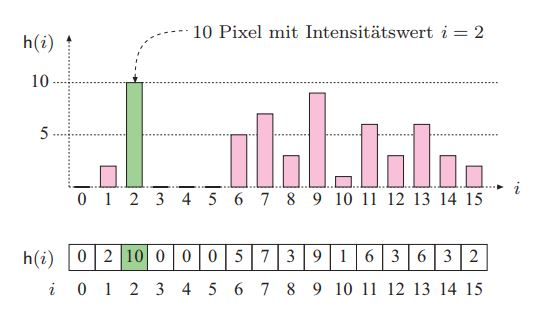
\includegraphics[scale=0.8]{Sources/histogramm.jpg}
    \caption{Histogramm eines Graustufen-Bildes mit 16 Helligkeitsabstufungen \cite[42]{burger2009digitale}}
    \label{img:histogramm}
  \end{figure}\\
Die Abbildung \ref{img:histogramm} zeigt ein mögliches Histogramm mit einer Farbabstufung von 16 Werten. Ein Histogramm zeigt die wichtigsten Eigenschaften eines Bildes, wie beispielsweise die Dynamik oder den Kontrast. Außerdem kann festgestellt werden, ob bei der Bildaufnahme Probleme aufgetreten sind. Diese Probleme lassen sich an ganz linken oder ganz rechten Ausschlägen des Graphen erkennen. Ein Ausschlag bei 0 oder 255 bedeutet, dass dort keine Farbinformationen mehr vorhanden sind und Teile des Bildes über- beziehungsweise unterbelichtet sind.\\\\
\textbf{Kontrast}\label{s.kontrast}\\
Der Kontrast bezeichnet den Bereich von Intensitätstufen, welche in einem Bild effektiv genutzt werden, also die Differenz der maximalen und minimalen Pixelwerte \cite[44]{burger2009digitale}. Ein Bild, welches einen hohen Kontrast hat, nutzt das gesamte Spektrum des Histogramms (Schwarz bis Weiß). Der Kontrast lässt sich also leicht aus einem Histogramm entnehmen, wie die verschiedenen Histogramme in Abbildung \ref{img:dynamik} zeigen.
  \begin{figure}
    [h]
    \centering
    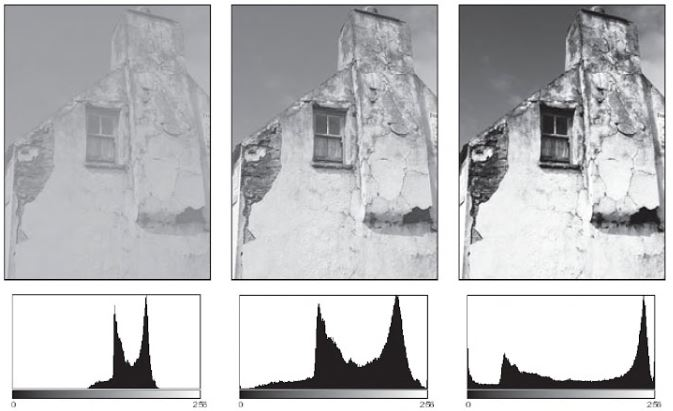
\includegraphics[scale=0.5]{Sources/kontrast.JPG}
    \caption{Unterschiedlicher Kontrast und die Auswirkungen im Histogramm: niedriger Kontrast (links), normaler Kontrast (Mitte), hoher Kontrast (rechts)\cite[45]{burger2009digitale}}
    \label{img:kontrast}
  \end{figure}
  \newpage
\textbf{Dynamik}\label{s.dynamik}\\
Dynamik beschreibt den Quotienen aus dem größten und dem kleinsten Intensitätswerten in einem Bild und deren jeweilige Anzahl \cite[44]{burger2009digitale}. Im besten Fall entspricht die Dynamik der insgesamt genutzten Anzahl an Pixelwerten (Abbildung \ref{img:dynamik}). Also $K-1$ genutzter Farbabstufungen, damit der Wertebereich voll ausgeschöpft wird.
 \begin{figure}
    [h]
    \centering
    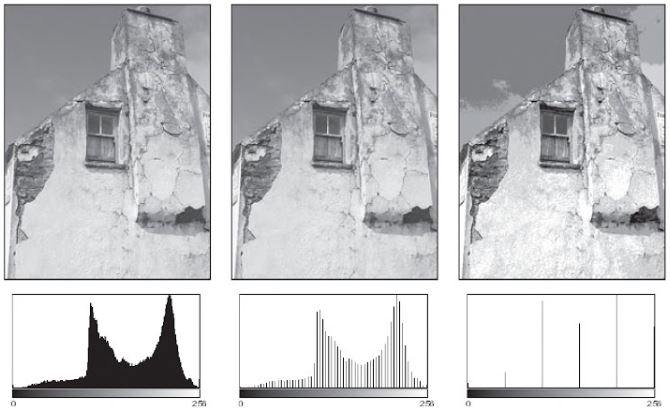
\includegraphics[scale=0.5]{Sources/dynamik.JPG}
    \caption{Unterschiedliche Dynamik und die Auswirkungen im Histogramm: hohe Dynamik (links), niedrige Dynamik mit 64 Graustufen (Mitte), extrem niedriger Kontrast mit 6 Graustufen (rechts)\cite[45]{burger2009digitale}}
    \label{img:dynamik}
  \end{figure}\\
Anders als der Kontrast, welcher immer erhöht werden kann, solange der maximale Wertebereich nicht erreicht worden ist, kann die Dynamik eines Bildes nicht so leicht verbessert werden. Aus diesem Grund ist eine hohe Dynamik von Vorteil, denn dadurch wird die Gefahr von Qualitätsverlust bei Verarbeitungsschritten verringert. Trotz der Tatsache, dass viele Ausgabegeräte mit Farbtiefen von 8 Bit arbeiten, nehmen heutige Kameras bis zu 12-14 Bit pro Kanal auf, um einem möglichen Qualitätsverlust vorzubeugen.
\subsection{Einfluss von Belichtungen}\label{s.belichtung}
In dem Unterabschnitt \ref{s.aufbdigibilder} wurde beschrieben, wie Farben in Bildern gespeichert werden und welche unterschiedlichen Arten von Farbräumen es gibt \cite[41ff.]{burger2009digitale}. Bei der Aufnahme von Bildern ist gerade die Belichtung entscheidend. Eine hohe Belichtung sorgt dafür, dass Farben heller wirken, wobei wenig Licht dafür sorgt, dass Farben dunkler erscheinen. Diese Tatsache kann beim Deep Learning zu Problemen führen, da ein und dasselbe Objekt unterschiedliche Farben annehmen kann und je nach Belichtungsintensität variiert. Ein künstliches neuronales Netz kann Objekte, welche es normalerweise trainiert hat, nicht immer erkennen, wenn die Farbe zu stark von der eigentlichen Farbe abweicht. Um Belichtungen auf Bildern auszugleichen und zu normalisieren, gibt es einige Verfahren, welche diesem Problem entgegenwirken. Ziel der Farbnormalisierung ist es nicht die Originalfarbe des Objektes wieder herzustellen, sondern für eine konstante Farbvariation zu sorgen. Die für diese Arbeit ausgewählten Verfahren werden im Abschnitt \ref{s.farbnormalisierungen} aufgeführt und beschrieben. 
\section{Künstliche Intelligenz}\label{s.ki}
In den letzten Jahren hat die Nutzung von künstlichen Intelligenzen enorm zugenommen. Viele Firmen nutzen diese Technologie beispielsweise für die Analyse und Vorhersage von Kundenverhalten, für die Klassifikation von Bildern oder für die Spracherkennung in heutigen Smartphones. Mit künstlicher Intelligenz beschreibt man Computer, welche gewisse Aufgaben erledigen, ohne ausdrücklich dafür programmiert worden zu sein. Dafür werden dem System Informationen anhand von Vergleichsdaten zugeführt, wodurch es sich Eigenschaften und Strukturen merkt und durch diese Rückschlüsse und Prognosen ziehen kann. Eine gute Beschreibung liefern dabei die Autoren Rich und Knight, indem sie schrieben:\\\\
 \textit{Das Studium des Problems, Computer dazu zu bringen, Dinge zu tun, bei denen ihnen momentan der Mensch noch überlegen ist.} - (Rich und Knight 1991) \cite[231]{kuppers2017humanoide}\\\\
Ein gutes Beispiel, in welchem man das Potenzial von künstlicher Intelligenz sehen kann, ist die Spiele-KI  \textit{AlphaGo}. Diese KI wurde von Google entwickelt und ist auf das Spielen des Brettspiels Go trainiert. So konnte \textit{AlphaGo} in einem Match 2016, den damaligen Weltmeister in Go \textit{Lee Sedol} schlagen \cite{Alpha2016GO}. In vier von fünf Spielen gewann der Computer. Solche Ergebnisse konnten bis zu diesem Zeitpunkt mit anderen Methoden nicht erzielt werden, da es für damalige Algorithmen zu viele mögliche Spielzüge gab. Durch Deep Learning konnte der Computer, ohne feste Algorithmen, seine Spielzüge besser als der Weltmeister planen \cite[331 ff.]{ertel2013grundkurs}. Anhand der Definition von Rich kann das  \textit{AlphaGo}  im Bereich des Spieles Go als intelligent bezeichnet werden, da es dem besten Go-Spieler der Welt deutlich überlegen war.
  \section{Neuronale Netze}\label{s.neuronalenetze}
Um das Konzept hinter den künstlichen neuronalen Netzen besser verstehen zu können, betrachten wir zunächst, wie der Lernprozess eines Menschen abläuft. Menschliches Lernen ist das Verändern der eigenen Verhaltensstrukturen aufgrund von individuellen Erfahrungen \cite{hoffmann2016lern}. Der Lernprozess kann sowohl bewusst sowie auch unbewusst unser Verhalten verändern. Menschen adaptieren also sowohl die eigenen, als auch fremde Erfahrungen zu ihren Gewohnheiten. Diese Prozesse finden im Gehirn statt, welches aus vielen Nervenzellen besteht. Diese Nervenzellen werden Neuronen genannt und sind untereinander verknüpft, weshalb auch von einem neuronalen Netz gesprochen wird. Maschinelles Lernen nimmt sich demnach die Funktionsweise des menschlichen Gehirns zum Vorbild \cite[1]{ertel2013grundkurs}.\\\\
\textbf{Menschliches Lernen}\\
Wie bereits erwähnt, sind der Aufbau sowie die Funktionsweise von künstlichen neuronalen Netzen vom menschlichen Gehirn abgeleitet. Das Gehirn besteht aus ungefähr $10^{11}$ Nervenzellen, welche untereinander verknüpft sind \cite[265ff.]{ertel2013grundkurs}. Für den Lernprozess sind demzufolge viele Neuronen nötig. In der Abbildung \ref{img:neuron} kann man den wesentlichen Aufbau eines Neurons sehen.
\begin{figure}
	[h]
	\centering
	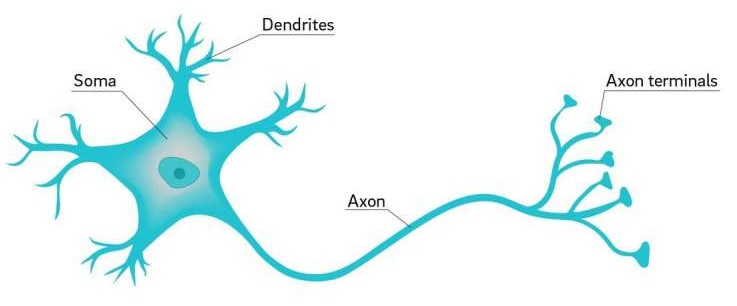
\includegraphics[scale=0.7]{Sources/neuron.jpg}
	\caption{Aufbau eines Neurons \cite{neuron2018UoC}}
	\label{img:neuron}
\end{figure}\\
In diesem vereinfachten Modell eines Neurons lassen sich dessen wesentliche Komponenten erkennen. Das Neuron selber besteht aus einem Zellkörper (Soma), einem Axon, den Dendriten auf der linken Seite und den Synapsen (Axon Terminals) auf der rechten Seite. Eine Dendrite stellt mit der Synapse eine Verbindung zu anderen Neuronen her. Sie sendet elektrische Impulse an die Soma weiter, welche dort verarbeitet werden. Wenn die Spannung einen gewissen Schwellwert übersteigt, sendet die Soma einen elektrischen Impuls über das Axon. Jede Synapse sendet das Signal an die Dendriten des nächsten Neurons weiter. Die Stärke des Impulses und der Schwellwert ist bei jedem Neuron unterschiedlich und sie verändern sich ständig. Der Schwellwert des Neurons ist niedriger, desto öfter es aktiv ist und steigt, wenn es selten aktiv ist \cite{schmidt2013physiologie}. Die aufgeführte Funktionsweise beschreibt nur oberflächlich das Verhalten eines neuronalen Netzes und soll hauptsächlich dem weiteren Verständnis dienen.\\
\textbf{Perzeptron}\\
Die Grundlage für den mathematischen Ablauf künstlicher neuronaler Netze wurde in dem Buch von McCulloch und Pitts \textit{A logical calculus oft he ideas immanent in nervous activity} erklärt \cite{McCulloch1943}. Auf diesen Grundlagen simulierte 1953 der Psychologe und Informatiker Frank Rosenblatt das erste künstliche Neuron, welches auch als Perzeptron bekannt wurde. In der Abbildung \ref{img:Perzeptron} wird der Aufbau eines solchen Perzeptrons dargestellt und Formell beschrieben \cite[269]{ertel2013grundkurs}.
\begin{figure}
	[h]
	\centering
	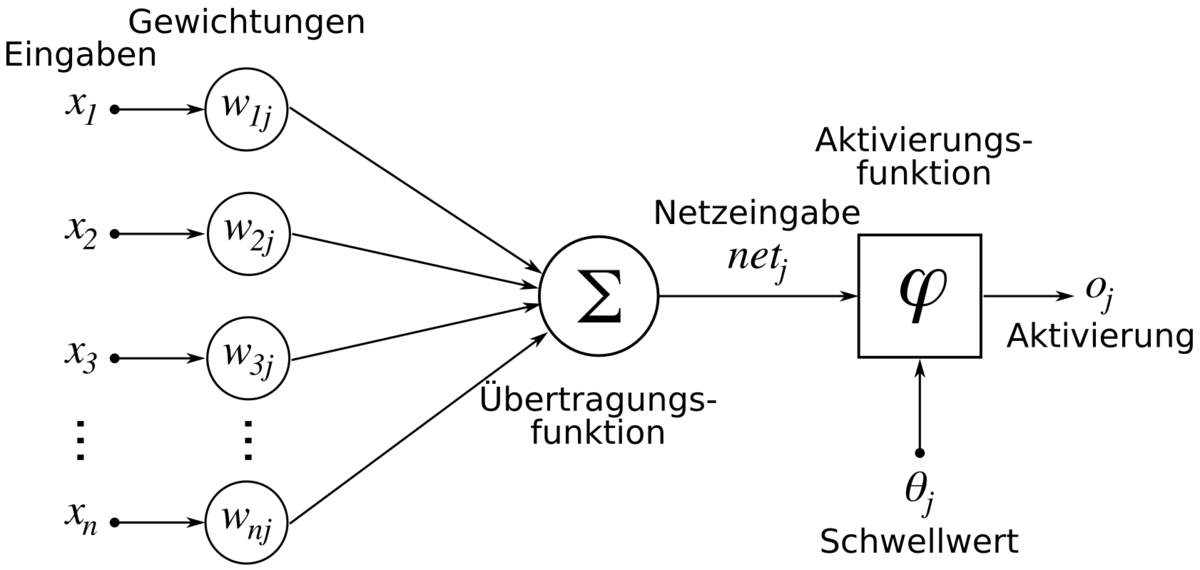
\includegraphics[scale=0.25]{Sources/perzeptron2.png}
	\caption{Schematische Modellierung eines Perzeptrons nach Rosenblatt \cite{perzeptron2019}}
	\label{img:Perzeptron}
\end{figure}
Als Eingabewert bekommt das Perzeptron ein Gewicht $w$, welches mit den Eingangswert $x$ multipliziert wird. Das Ergebnis dieser beiden Werte, kann als lineare Funktion beschrieben werden.
\begin{eqnarray} f(x) & = & w*x \end{eqnarray}
Anschließend wird das Ergebnis der beiden Werte an eine Aktivierungsfunktion $g$ übergeben. Die Aktivierungsfunktion oder auch Schwellwert genannt gibt ein Signal weiter, sobald dieser Wert überschritten wird.
\begin{eqnarray} g( \sum_{i=0}^n x_{i} *w_{i}) \end{eqnarray}
Als Aktivierungsfunktion können sowohl lineare als auch nicht linearen Funktionen verwendet werden. Zusätzlich wird dem Ergebnis der Funktion der \textit{Bias} $b$ dazu addiert.
\begin{eqnarray} g(( \sum_{i=0}^n x_{i} *w_{i}) +b) \end{eqnarray}
Der \textit{Bias} ist eine Art zusätzliches Neuron für das Verringern von Konvergenz-Problemen, welche bei der Approximation der Funktion auftreten können. Der Bias hat immer einen Eingabewert von 1 und ein Gewicht $w_{bias}$, welches unabhängig von den Eingabewerten ist.
\begin{eqnarray} Bias = 1*w_{bias} \end{eqnarray}
Maschinelles Lernen möchte unter anderem Maschinen dazu in die Lage versetzen Objekte, Strukturen oder auch Abläufe anhand von vorher beigebrachten Beispielen eigenständig zu erkennen. Eine Methode, um dieses Ziel erreichen zu können, sind die künstlichen neuronalen Netze. Diese werden mit Datensätzen des jeweiligen Schwerpunktes trainiert. Es gibt vier grundlegende Methoden ein solches Netz zu trainieren \cite[694ff.]{russell2016artificial}.\\\\
\textbf{Überwachtes Lernen}\\
Das überwachte Lernen (superviced learning) funktioniert hauptsächlich mit Datensätzen, welche Eingabedaten sowie Ausgabedaten enthalten. Das künstliche neuronale Netz versucht bei Eingabe der Daten eine Funktion aufzustellen, welche eine Hypothese darstellt. Diese beschreibt, um was es sich bei dem Datensatz handelt. Die Genauigkeit dieser Hypothese kann durch den Vergleich der enthaltenden Ausgabedaten ermittelt werden. Wenn die Möglichkeiten der Ausgaben endlich sind, handelt es sich um eine Klassifizierung (Bsp.: Milch, Orangensaft, Wasser, etc.). Sollten nur zwei Ausgabewerte möglich sein, ist es eine boolsche bzw. binäre Klassifizierung. Eine Zahl als Ausgabe wird als Regression bezeichnet.
\newpage
\textbf{Nicht überwachtes Lernen}\\
Die zweite Methode (unsuperviced learning), wie ein künstliches neuronales Netz trainiert werden kann, ist eine gegenteilige Herangehensweise. Hier werden lediglich die Eingabedaten übergeben. Das neuronale Netz versucht selbstständig auftretende Muster in den Daten zu erkennen. Als Beispiel könnte man die sinnvolle Zuordnung von Bildern anhand ähnlicher Muster nehmen. Ähnliche Datensätze werden in Kategorien aufgeteilt, jedoch nicht benannt.\\\\
\textbf{Halb überwachtes Lernen}\\
Oft werden die beiden Methoden des überwachten und unüberwachten Lernen kombiniert (semi-superviced learning). So hat man meist einen Teil mit Ein- und Ausgabedaten, welche nicht explizit wahr sein müssen und einen anderen Teil nur mit Eingabeinformationen. Diese Methode wird häufig bei Umfragen verwendet, wo nicht klar ist, ob der Proband wahrheitsgemäß antwortet. Dabei kann ein systematischer Fehler entstehen. Daraus ergibt sich eine Mischung aus überwachtem Lernen mit systematischen Fehler und unüberwachtem Lernen, bei welchem das Netz nach häufig auftretenden Mustern sucht.\\\\
\textbf{Bestärkendes Lernen}\\ 
Das bestärkende Lernen (reinforcment learning) arbeitet nach einem Prinzip, bei dem richtige Entscheidungen belohnt und falsche bestraft werden. Ein bekanntes Beispiel ist ein Netz, welches virtuell eine Rennstrecke ohne Fehler (nicht von der Strecke abkommen) beenden muss. Bei jedem Fehler muss von vorne begonnen werden, bis die Strecke beendet wird. Ein besonders bekanntes Beispiel ist die Go-KI \textit{AlphaGo} \cite{Alpha2016GO}, welche nur durch die Informationen der Spielregeln trainiert wurde.\\\\
\textbf{Künstliche neuronale Netze}\\
Nachdem auf die Grundlagen der verschiedenen Lernverfahren eingegangen wurde, soll in diesem Abschnitt der Aufbau künstlicher neuronaler Netze (KNN) fokussiert werden. Der mathematische Ablauf der Schichten wird in einem späteren Unterkapitel behandelt.
\begin{figure}
	[h]
	\centering
	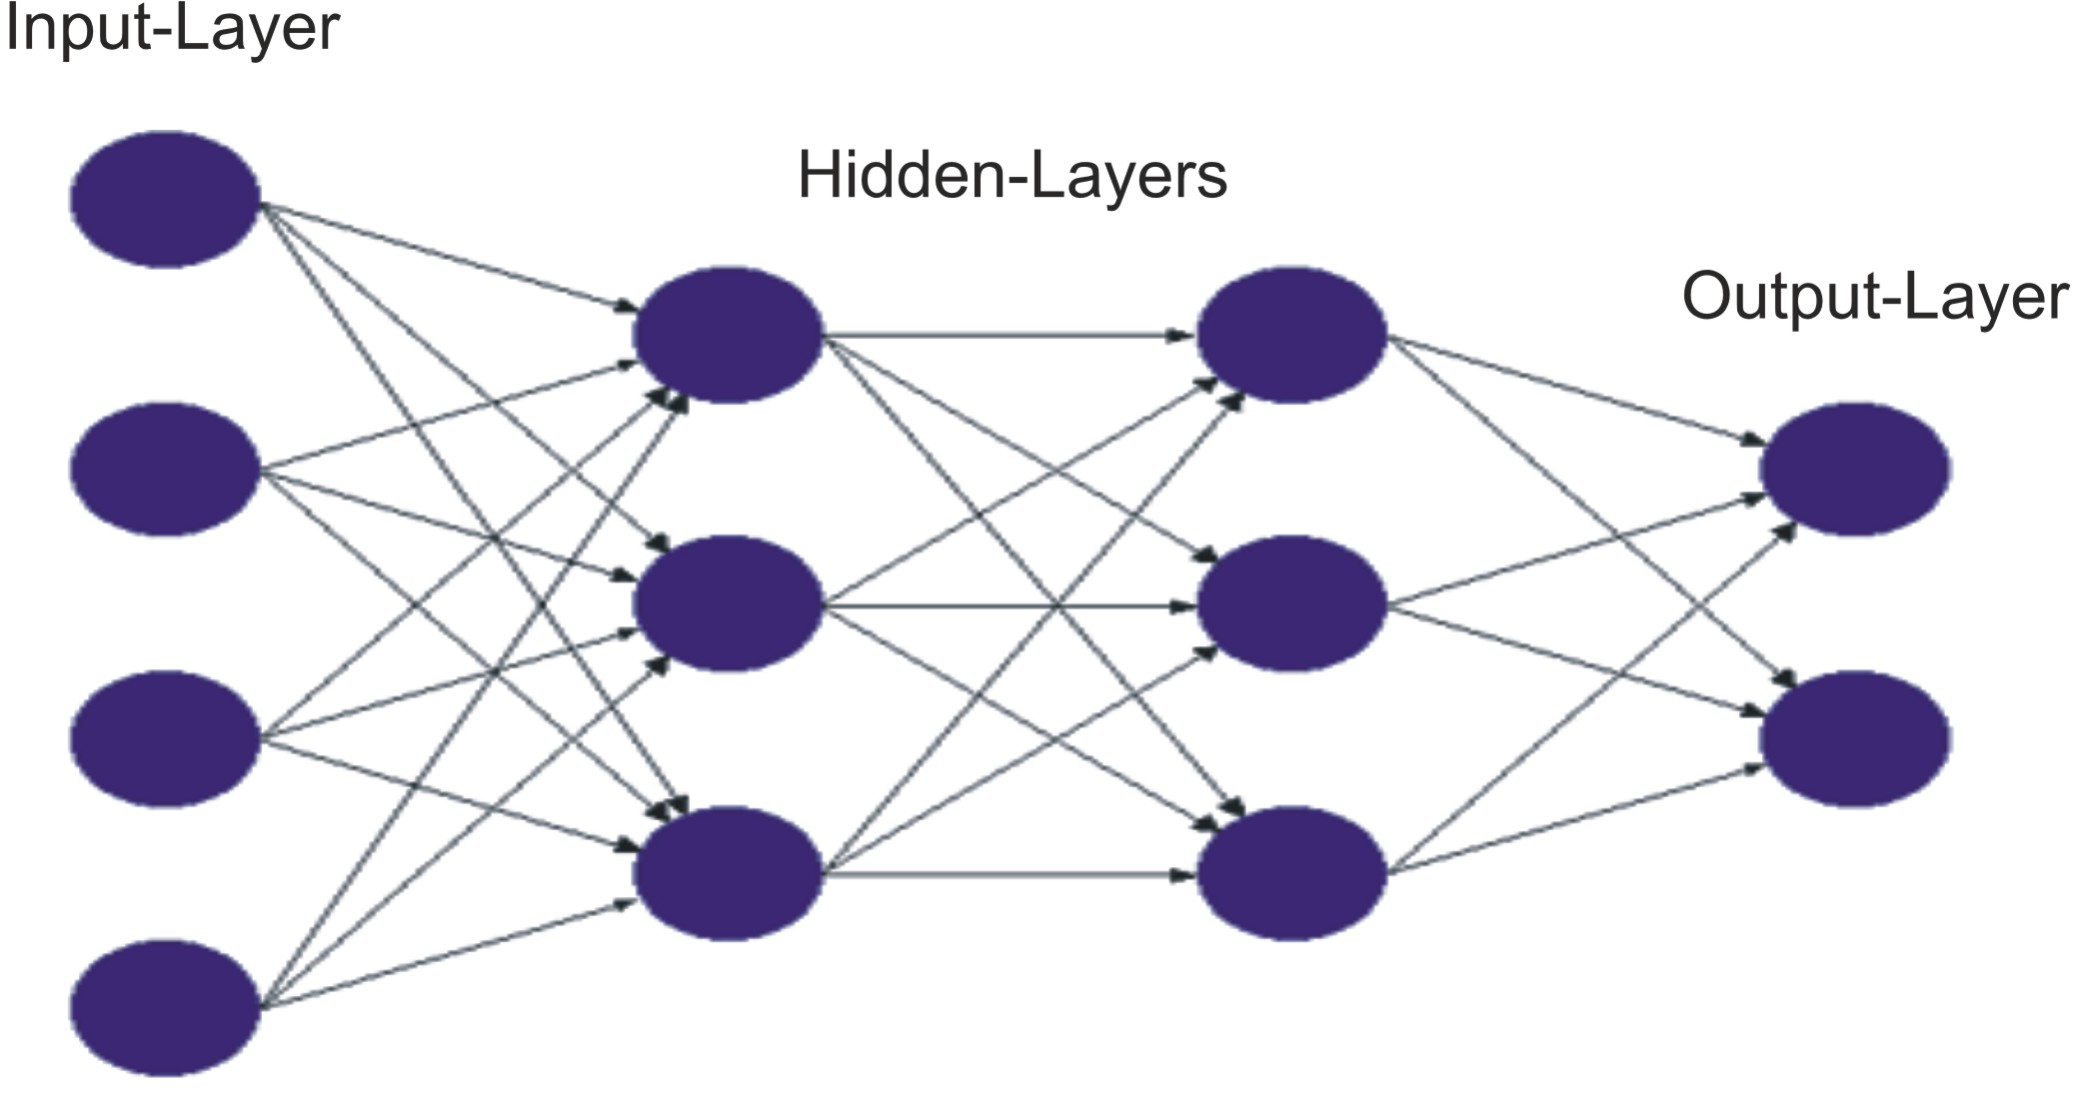
\includegraphics[scale=0.5]{Sources/nnet.png}
	\caption{Aufbau eines künstlichen neuronalen Netzes \cite{bistra2018pic}}
	\label{img:neuronales_netz}
\end{figure}
Der Aufbau von klassischen künstlichen neuronalen Netzen kann grundsätzlich in drei Bereiche unterteilt werden. Die erste Schicht stellt der \textit{Input Layer} dar. Dieser besteht, wie alle folgenden Schichten auch, aus mehreren Neuronen. In dieser Schicht werden die Trainingsdaten eingegeben. Jeder Wert eines Datensatzes wird mit einem Neuron verbunden. Die Neuronen besitzen eine Gewichtung und einen Schwellwert. Wenn der Schwellwert durch den Eingabewert erreicht wird, sendet das Neuron das Ergebnis seiner Berechnungen an das Neuron der nächsten Schicht weiter. Die folgenden Schichten werden \textit{Hidden Layer} genannt. Die Anzahl der \textit{Hidden Layer} ist variabel und kann so viele Schichten enthalten, wie benötigt werden. Diese Schichten werden auf mehrere verschiedene Merkmale der Eingabedaten trainiert. Dabei werden in den frühen Schichten zunächst grobe Strukturen erkannt, welche nach jeder weiteren Schicht immer feiner werden. Die letzte Schicht des \textit{Hidden Layer} übergibt seine Informationen an den \textit{Output Layer}. Dieser stellt durch die erhaltenen Daten eine Hypothese auf, in welcher er beschreibt, wie er den Datensatz zuordnet. Dabei gibt das Netz an, zu welcher Wahrscheinlichkeit die Hypothese richtig sein sollte.\\\\
\textbf{Faltende neuronale Netze}\label{s.cnn}\\
\textit{Convolutional neural Networks} oder auch faltende neuronale Netze (Abbildung \ref{img:cnn}) sind, anders als das künstliche neuronale Netz, an das Konzept des menschlichen Sehens angelehnt \cite{sermanet2012convolutional} und für das Verarbeiten von matrixartigen Datensätzen konzipiert. Dazu zählen beispielsweise Bildaufnahmen \cite{goodfellow2016deep}. Die erste Schicht besteht aus dem \textit{Convolutional Layer}. Bei dieser Schicht wird über die Pixel des Eingabebildes eine Schablone gelegt und vertikal wie auch horizontal verschoben. Diese Schablone hat eine ungerade quadratische Abmessung ($3x3$, $5x5$, $7x7$) und eigene Gewichtungen. Sie bildet ein Skalarprodukt der unterliegenden Pixel und der Gewichtung. Dabei werden die Strukturen hervorgehoben. Diese Schicht kommt mehrmals in einem Netz vor.\\  
\begin{figure}
	[h]
	\centering
	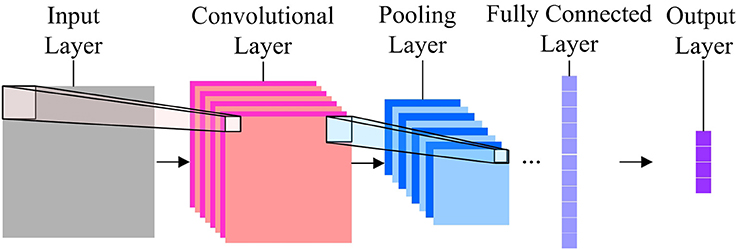
\includegraphics[scale=0.5]{Sources/cnnet.jpg}
	\caption{Aufbau eines Convolutional neural Network \cite{info7040061}}
	\label{img:cnn}
\end{figure}\\
Auf den \textit{Convolutional Layer} folgt immer der \textit{Pooling Layer}. Dieser ist für die Komprimierung des Eingabebildes zuständig, damit im späteren Verlauf Rechenleistung gespart werden kann. Auch diese Schicht besteht aus einer Schablone, welche über die Pixel des Bildes gelegt wird. Hierbei werden die Farbwerte der unterliegenden Pixel verarbeitet. Diese werden zu einem Wert zusammengefasst und übergeben. Nachdem alle \textit{Convolutional-} und \textit{Pooling Layer} durchlaufen wurden, werden die Daten an die letzte Schicht (\textit{Fully Connected Layer}) übergeben. Der \textit{Fully Connected Layer} besteht, wie beim KNN beschrieben, aus mehreren Perzeptronen-Schichten und gibt die Informationen an den \textit{Output Layer} weiter. Schlussendlich gibt dieser eine Hypothese mit der dazugehörigen Wahrscheinlichkeit aus.\\\\
\textbf{Loss Funktion}\\
Bei jedem Trainingsschritt versucht das neuronale Netz eine Hypothese aufzustellen. Für den Lernfortschritt des Netzes ist das sogenannte Backpropagation, welches im nächsten Abschnitt genauer beschrieben wird, zuständig. Es arbeitet auf der Basis des Loss Graphen. Die Loss Funktion berechnet den Fehler, welchen das Netz in seinem aktuellen Zustand in der Berechnung begeht, also die Differenz zwischen dem Ist- und Sollwert der Ausgabe. Ein Beispiel einer solchen Funktion, ist die euklidische Loss-Funktion:
\begin{eqnarray} E_{Euclid}&=&\frac{1}{2N} \sum_{n=1}^N || \hat{f_{n}}-f_{n} || \binom{2}{2} \end{eqnarray}
Dabei stellt
\begin{itemize}
	\item[] $\hat{f}_{n} \in [-\infty,+\infty]$ den berechneten Ist-Wert und
	\item[] $f_{n} \in [-\infty,+\infty]$ den Sollwert dar.
\end{itemize}
Das Ergebnis der euklidischen Funktion ist das Maß für den Grad der Abweichung von Ist- und Sollwert.\\\\
\textbf{Rückpropagierung}\\
Die Rückpropagierung oder auch \textit{Backpropagation} \cite{ertel2013grundkurs} ist unter anderem Teil des überwachten Lernens und beinhaltet das Lernen aus Fehlern. Dadurch, dass bei einer Klassifizierung Datensätze mit einem Zielwert verwendet werden, kann das Netz bei einer Zuweisung überprüfen, ob das Ergebnis zu dem Zielwert passt. Dabei wird aus der Ausgabe und dem Zielwert ein Fehler (Loss) berechnet. Sollte das Ergebnis zu weit vom Zielwert abweichen, wird überprüft, welches Perzeptron den größten Einfluss auf die Fehlzuweisung verursacht hat. Dieses Perzeptron wird in seiner Gewichtung angepasst, um den Fehlerwert zu verringern \cite{goodfellow2016deep}.\\\\  
\textbf{Funktionsweise künstlicher und faltender neuronaler Netze}\label{s.funktwknnundcnn}\\
Die zuvor aufgeführten Netzarten haben einen unterschiedlichen Aufbau und bestimmte Einsatzgebiete. Das Convolutional neural Network ist beispielsweise für das Verarbeiten von Bilddaten optimiert und künstliche neuronale Netze eher für das von seriellen Daten. In ihrer Struktur sind die Netzarten ähnlich aufgebaut. Das \textit{Convolutional neural Network} hat neben den üblichen Neuronenschichten zwei zusätzliche Schichten, welche beim künstlichen neuronalen Netz nicht vorhanden sind. In den folgenden Absätzen soll die Funktionsweise dieser zusätzlichen Schichten beschrieben werden\cite[343]{goodfellow2016deep}.\\\\
\textbf{Faltungsschicht}\\
Es existiert eine Menge von Filtern $n$, welche eine Höhe von $f_{h}$ und eine Breite von $f_{w}$ haben. Diese Filter werden über das Eingabebild mit der Höhe $e_{h}$ und der Breite $e_{w}$ gelegt und in 1-Pixel-Schritten bewegt. Die Ergebnisse stellen eine Liste von Merkmalen dar, welche auf der Höhe $m_{h}$ und der Breite $m_{w}$ liegen. In Formeln ausgedrückt:
\begin{eqnarray} 
m_{h}&=&(e_{h} - f_{h})+1\\
m_{w}&=&(e_{w} - f_{w})+1
\end{eqnarray}
Um die Verringerung von Informationen nach der Faltung zu verhindern, werden an den Rändern der Bilder Polsterungen, auch \textit{padding} genannt, angehangen \cite[343]{goodfellow2016deep}. Diese Polsterungen bestehen aus Pixeln mit einem Wert von \textit{0}. Die Anzahl der zusätzlichen Pixel ergibt sich aus der Höhe und Breite des Eingabebildes. In Formeln ausgedrückt:
\begin{eqnarray}
p_{h}&=&f_{h} - 1\\
p_{w}&=&f_{w} - 1
\end{eqnarray}
Die Faltungsschicht hat eigene Gewichte, welche beim Vorgang mit denen des Bildes zusammengerechnet werden \cite[331ff.]{goodfellow2016deep}. Für die gleiche Schicht wird derselbe Filter verwendet. Die Weise der Berechnung wird in der Abbildung \ref{img:faltungsschicht}  beschrieben.
\begin{figure}
	[h]
	\centering
	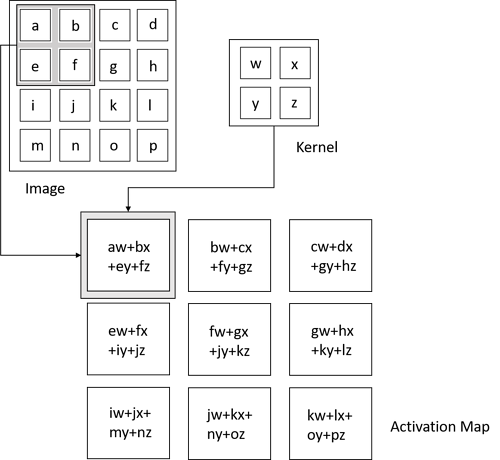
\includegraphics[scale=0.55]{Sources/CNN.png}
	\caption{Funktionsweise der Faltungsschicht \cite[330]{goodfellow2016deep}}
	\label{img:faltungsschicht}
\end{figure}
\newpage
\textbf{Pooling Schicht}\\
Die Pooling Schicht oder auch \textit{Pooling Layer} kommt nach jeder Faltungsschicht \cite[336f.]{goodfellow2016deep}. Die Aufgabe dieser Schicht ist es, das Eingabebild in der Auflösung und den zugehörigen Rechenaufwand für die folgenden Schichten zu reduzieren. Üblicherweise gibt es zwei Verfahren, welche beim Pooling eingesetzt werden. Zum einen das Average Pooling und das am häufigsten verwendete Max Pooling (Abbildung \ref{img:maxpooling}). Auch diese Schicht besteht aus einem quadratischen Filter, welcher wie bei der Faltungsschicht über die Bildpunkte gelegt wird. Dabei wird beim \textit{Max Pooling} der höchste Wert in diesem Bereich ermittelt und übernommen. Bei einem standardmäßigen Kernel von 2x2, wird das Bild um den Faktor 2 verkleinert. Die Abmessungen sind, anders als bei der Faltungsschicht, gerade.
\begin{figure}
	[h]
	\centering
	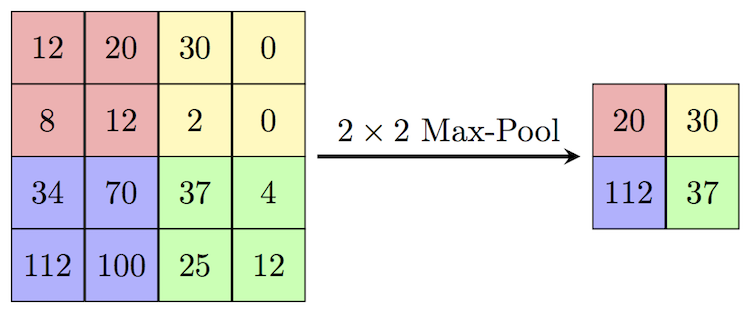
\includegraphics[scale=1.3]{Sources/MaxpoolSample2.png}
	\caption{Funktionsweise des Pooling Layers mit der Max Pooling-Variante \cite{pooling2018layer}}
	\label{img:maxpooling}
\end{figure}\\
\textbf{Fully connected Layer}\\
Nachdem das Eingabebild durch alle Faltungs- und Pooling-Schichten verarbeitet wurde, werden die Daten an den Fully connected Layer übergeben \cite[14]{sermanet2012convolutional}. Dieser verwendet, wie bei einem normalen KNN, Perzeproten, um die Daten zu verarbeiten. Die vorherigen Schichten wurden durchlaufen, damit diese rechenintensive Schicht nicht zu viele Informationen verarbeiten muss. 
  \subsection{Entstehung von Trainingsdaten}\label{s.trainingsdaten} 
Damit ein künstliches neuronales Netz Objekte erkennen und zuordnen kann, benötigt es zunächst eine Reihe von Beispieldaten. Anhand dieser Beispieldaten lernt das neuronale Netz, welche Eigenschaften das zu erlernende Objekt hat und wie es aufgebaut ist. Für diesen Vorgang werden üblicherweise mehrere hunderttausend Daten benötigt, um ein akzeptables Ergebnis zu erzielen. Eine Möglichkeit, das Training mit weniger Trainingsdaten durchzuführen, ist das Verwenden vortrainierter Netze. Diese Netze wurden mit rund 300.000 Bildern über mehrere Tage trainiert und als Open Source zur Verfügung gestellt. Beim Verwenden dieser Netze werden lediglich die obersten Schichten, welche für die Zuweisung verantwortlich sind, durch den neuen Datensatz verändert, wodurch wesentlich weniger Testdaten pro Objektklasse benötigt werden. 
\begin{figure}
	[h]
	\centering
	\setlength{\fboxsep}{1pt} 
    \setlength{\fboxrule}{1pt}
	\fbox{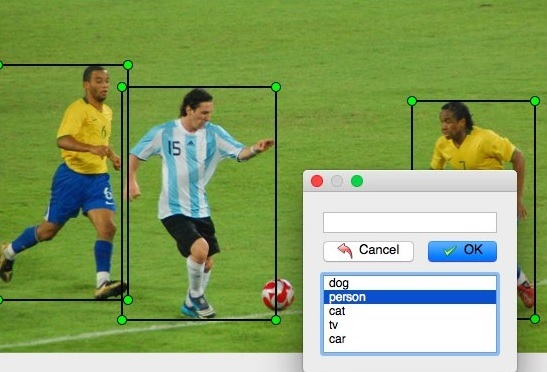
\includegraphics[scale=0.6]{Sources/labelimg.jpg}}
	\caption{Vorbereitung der Datensätzen mit dem Labeling-Programm \cite{labelimg2019}}
	\label{img:labelimg}
\end{figure}
Eine Klassifizierung gehört zum überwachten Lernen und benötigt deswegen gelabelte Datensätze. Das Labeln wurde mit dem Open-Source-Programm \textit{LabelIMG} \cite{labelimg2019} durchgeführt. Hierbei wird das zu trainierende Objekt mit einem rechteckigen Kasten umschlossen und mit einer Klasse auf den Bildern markiert. Diese Daten werden zunächst in einer XML-Datei abgespeichert. 
  \subsection{Mean average Precision}\label{s.map}
Oft können neuronale Netze nicht nur ein Objekt erkennen, sondern geben als Ergebnis mehrere Hypothesen aus. Dadurch entsteht das Problem, dass nicht mehr nur zwischen richtig und falsch unterschieden werden kann, sondern eine Genauigkeit benötigt wird, welche alle möglichen Objekte einbezieht. Eine Metrik, welche auf diese Informationen eingeht, ist die (mean) average Precision (AP/mAP) \cite{map2019hui}. Für die Berechnung wird die Präzision (Precision) und der Rückgabewert eines Ergebnisses benötigt. Die Präzision $P$ beschreibt den Anteil der richtig erkannten Objekte unter allen erkannten Objekten. Der Rückgabewert $R$ (Recall) ist der korrekte Anteil von allen möglichen Objekten. In Formeln ausgedrückt:
\begin{eqnarray}
P&=&\frac{richtig\medspace erkannte}{richtig\medspace erkannte + falsch\medspace erkannte}\\
R&=&\frac{richtig\medspace erkannte}{richtig\medspace erkannte + falsche\medspace nicht\medspace erkannte}
\end{eqnarray}
Häufig wird ein Schwellwert für die Pseudowahrscheinlichkeit genutzt, mit welchem entschieden wird, wann ein erkanntes Objekt der Rückgabeliste hinzugefügt wird oder nicht. Wird der Schwellwert niedrig angesetzt, werden meist mehr Objekte als \textit{erkannt} eingestuft. Dadurch steigt der Rückgabewert mit richtig erkannten Objekten. Gleichzeitig sinkt aber auch die Präzision, da natürlicherweise auch mehr falsche Objekte erkannt werden. Objekterkennungsverfahren mit einer hohen Qualität haben aber weiterhin eine hohe Präzision.
\section{Arten der Farbnormalisierung}\label{s.farbnormalisierungen}  
Die Farbnormalisierung ist ein Thema der Bildverarbeitung, welches sich hauptsächlich mit künstlicher Farbsicht befasst. Die Verteilung und Darstellung von Farben auf Bildern hängt hauptsächlich von Beleuchtungsbedingungen und der Kamera ab. Das bedeutet, dass sich die Farben bei der Aufnahme, je nach Beleuchtung, verändern. Das ist gerade im Bereich von \textit{Machine Learning} problematisch, da diese Farbveränderungen zu Fehlern im Lernprozess und der späteren Genauigkeit führen. Farbnormalisierungs-Algorithmen sollen dafür sorgen, dass die Farbabweichungen durch Lichteinfluss geringere Auswirkungen haben und zu besseren Ergebnissen führen. Im Folgenden werden die ausgewählten Algorithmen erläutert, welche im Rahmen dieser Arbeit getestet werden.
  \subsection{Ansatz des Gray-World-Algorithmus}\label{s.gw}
Bei der Gray-World-Normalisierung \cite{buenaposada2001variations} geht es nicht, wie der Name vermuten lässt, um die Umwandlung in ein Graustufenbild, eher werden die verschieden Farbräume abgedunkelt und eingegrenzt. Wenn über die Farben in einem Bild keine Annahmen getroffen werden können, wird davon ausgegangen, dass die Farbwerte in einem Bild sich vektoriell zu Grau addieren, also das der Mittelwert vom Bild Grau ist. Sollte dies nicht der Fall sein, wird davon ausgegangen, dass das auf eine farbige Beleuchtung zurückzuführen ist und normalisiert das Bild so, dass die Graue-Welt-Theorie erfüllt wird. Die Farbkanäle werden durch einen Skalierungsfaktor normalisiert so, dass der Mittelwert 128 entspricht. Es werden somit Farbstiche herausgefiltert. Wie schon erwähnt, ist diese Art der Farbnormalisierung für verschiedene Farbvariationen unveränderlich. Ein Problem dieses Normalisierungsverfahrens besteht darin, dass es nicht einfach für dynamische Szenen verwendet werden kann. Um solche Probleme zu lösen, gibt es mehrere Ansätze dieser Ausgleichung.
\begin{align} \label{f:gw} (\alpha R, \beta G, \gamma B) \rightarrow\left(\frac{\alpha R} {\frac{\alpha}{n} \sum_{i} R}, \frac{\beta G} {\frac{\beta}{n} \sum_{i} G}, \frac{\gamma B} {\frac{\gamma}{n} \sum_{i} B} \right) \end{align}
Eine Veränderung der Beleuchtungsfarbe kann als Skalierung von $\alpha$, $\beta$ und $\gamma$ für die R-, G- und B-Kanäle modelliert werden (\ref{f:gw}). Als solcher ist der Gray-World für die Variationen der Beleuchtungsfarbe unveränderlich. Dieses Vorgehen berücksichtigt aber nicht alle Intensitäten der Beleuchtungsintensität und ist nicht für dynamische Szenen geeignet. Aus diesem Grund gibt es verschiedenste Ansätze dieses Verfahrens.
  \subsection{Ansatz der Histogramm-Ausgleichung}\label{s.ha}  
Die Histogramm-Ausgleichung \cite{goatman2003colour} ist eine nichtlineare Transformation, welche auf Grundlage der Histogramme arbeitet. Der Pixelrang wird dabei nicht verändert und kann bei jeder monoton steigenden Farbformation verwendet werden. Dieses Normalisierungsverfahren wird besser als der Gray-World-Algorithmus angesehen, da nicht nur die Farbkanäle beeinflusst werden, sondern auch die Farbverteilung in den Bildern. Durch die Histogramm-Ausgleichung entsteht ein dominanter blauer Kanal, wodurch das Bild oft unnatürlich erscheint.
   \begin{table}
  [h]
  \centering
  \caption{Pixelbild in ein tabellarisches Histogramm überführt}
  \label{tab:bildha}
  \begin{minipage}{\textwidth}
  \center
  \begin{tabular}{|c|c|c|c|c|c|c|c|}
  \hline
  0&1&5&1&7&2&0&3\\
  \hline
  0&0&5&5&5&2&4&5\\
  \hline
  4&5&1&4&1&5&1&4\\
  \hline
  5&1&2&4&5&2&6&3\\
  \hline
  5&2&6&4&0&4&0&5\\
  \hline
  4&0&2&4&7&4&6&2\\
  \hline
  5&1&6&1&0&1&1&5\\
  \hline
  4&5&2&4&2&5&2&5\\
  \hline
  \end{tabular}
  \end{minipage}
  \begin{minipage}{\textwidth}
  \hspace{\textwidth}
  \end{minipage}
  \begin{minipage}{\textwidth}
  \center
  \begin{tabular}{|l|c|c|c|c|c|c|c|c|}
  \hline
  Graustufen & 0 & 1 & 2 & 3 & 4 & 5 & 6 & 7\\
  \hline
  Anzahl der Pixel & 8 & 10 & 10 & 2 & 12 & 16 & 4 & 2\\
  \hline
  \end{tabular}
  \end{minipage}
  \end{table}
Für die mathematische Herleitung betrachten wir zunächst ein Graustufenbild $X$ und geben mit $n_{i}$ die Anzahl der Graustufen an, wobei $i$ die Häufigkeit des auftretenden Pixels ist. Zu sehen ist dies in der Funktion \ref{f:ha1}.
\begin{eqnarray} \label{f:ha1} p_{x}(i)=p(x=i)&=&\frac{n_{i}}{n}, 0\leq i \leq L \end{eqnarray}
$L$ ist die Gesamtzahl aller Graustufen im Bild (normalerweise 256), $n$ ist die Gesamtzahl der Pixel im Bild und $p_{x}(i)$ das normalisierte Histogramm für den Pixelwert $i$. Die Definition der Verteilungsfunktion kann man in \ref{f:ha1} sehen:
\begin{eqnarray} cdf_{x}(i) &=& \sum_{j=0}^i p_{x}(j)\end{eqnarray}
Um die Funktionsweise etwas verständlicher zu machen, folgt ein Beispiel in Form eines 8x8-Bildes (Tabelle \ref{tab:bildha}) mit acht Graustufen. Die Pixelverteilung wird in dem tabellarischen Histogramm zusammengefasst.  
Aus der Pixelverteilung wird nun ein Ausgleich berechnet, welcher den kumulativen Pixelwert durch die Anzahl aller Pixel teilt und das Ergebnis wiederum durch die höchste Graustufe. Das wird für jede Grauabstufung durchgeführt, wie in Tabelle \ref{tab:haberechnung} beschrieben.
 Das Ergebnis wird nun gerundet und der passenden Graustufe zugeordnet. Die Vorgehensweise mit Farbbildern ist, abgesehen davon, dass die R-, G- und B-Kanäle verwendet werden, gleich. Häufig wird für diese Verfahren ein Farbraum gewählt, welcher einen Kanal für die Luminanz besitzt.
  \begin{table}
  [h]
  \caption{Mathematische Umsetzung der Histogrammausgleichung}
  \label{tab:haberechnung}
  \centering
  \begin{tabular}{|l|c|c|c|c|}
  \hline
  $r_{k}$&$P_{k}$&Kumulative Werte&$Kumulative/Gesamt*(L-1)$&Gerundete Grauwerte\\
  \hline
  0 & 8 & 8 & $8/64*7=0.875$ & 1\\
  \hline
  1 & 10 & 18 & $18/64*7=1.968$ & 2\\
  \hline
  2 & 10 & 28 & $28/64*7=3.0625$ & 3\\
  \hline
  3 & 2 & 30 & $30/64*7=3.2812$ & 3\\
  \hline
  4 & 12 & 42 & $42/64*7=4.5937$ & 5\\
  \hline
  5 & 16 & 58 & $58/64*7=6.3437$ & 6\\
  \hline
  6 & 4 & 62 & $62/64*7=6.78125$ & 7\\
  \hline
  7 & 2 & 64 & $64/64*7=7$ & 7\\
  \hline
  \end{tabular}
  \end{table}
Die Graustufen werden im nächsten Schritt übernommen und in das Quellbild eingesetzt. Hierbei verschieben sich die Grauwerte so, dass sie den gerundeten Grauwerten aus Tabelle \ref{tab:haberechnung} entsprechen. Das ausgeglichene Bild kann man in der Tabelle \ref{tab:hamatrix} betrachten. 
\begin{table}[htb]
  \caption{Bildmatrix des ausgeglichenen Histogramms}
  \label{tab:hamatrix}
  \centering
  \begin{minipage}{\textwidth}
  \center
  \begin{tabular}{|c|c|c|c|c|c|c|c|}
  \hline
  1&2&6&2&7&3&1&3\\
  \hline
  1&1&6&6&6&3&5&6\\
  \hline
  5&6&2&5&2&6&2&5\\
  \hline
  6&2&3&5&6&3&7&3\\
  \hline
  6&3&7&5&1&5&1&6\\
  \hline
  5&1&3&5&7&5&7&3\\
  \hline
  6&2&7&2&1&2&2&6\\
  \hline
  5&6&3&5&3&6&3&6\\
  \hline
  \end{tabular}
  \end{minipage}
  \begin{minipage}{\textwidth}
  \hspace{\textwidth}
  \end{minipage}
  \begin{minipage}{\textwidth}
  \center
  \begin{tabular}{|l|c|c|c|c|c|c|c|c|}
  \hline
  Graustufen & 0 & 1 & 2 & 3 & 4 & 5 & 6 & 7\\
  \hline
  Anzahl der Pixel & 0 & 8 & 10 & 12 & 0 & 12 & 16 & 6\\
  \hline
  \end{tabular}
  \end{minipage}
  \end{table}
  \subsection{Ansatz der Histogramm-Spezifikation}\label{s.hs}
Ähnlich wie die Histogramm-Ausgleichung arbeitet die Histogramm-Spezifikation\\ \cite{goatman2003colour}. Die Histogramme der roten, grünen und blauen Kanäle werden so umgewandelt, dass sie den Formen von drei spezifischen Histogrammen entsprechen, anstatt sie einfach auszugleichen. Mithilfe dieses Vorgehens wird darauf abgezielt, Bilder zu erhalten, welche ein Histogramm einer bestimmten Farbverteilung haben. Zunächst muss das Bild so konvertiert werden, dass das Histogramm eine bestimmte Farbverteilung hat. Für diese Methode werden üblicherweise zwei ähnliche Bilder verwendet, das Quell- und das Referenzbild. Das Referenzbild hat die gewünschte Form des Histogramms, wohingegen das Quellbild angepasst werden soll. Häufig wird zunächst eine Histogramm-Ausgleichung der beiden Bilder durchgeführt. Sie kann aber auch mit den Originalbildern durchgeführt werden. Im Weiteren wird das Histogramm des Quellbildes auf das Histogramm des Referenzbildes angepasst. Die mathematische Herleitung beginnt auch hier mit einem Grasstufeneingabebild $S$. 
Dieses Bild hat eine Wahrscheinlichkeitsdichtefunktion $p_{r}(r)$, wobei $r$ ein Graustufenwert ist und $p_{r}(r)$ die Wahrscheinlichkeit für diesen Wert darstellt. Aus dem Histogramm des Bildes, kann die Wahrscheinlichkeit berechnet werden:
\begin{eqnarray} p_{r}(r_{j})&=&\frac{n_{j}}{n} \end{eqnarray}
Dabei ist $n_{j}$ die Frequenz des Graustufenwerts $r_{j}$ und $n$ die Gesamtzahl der Pixel im Bild. Bei Betrachtung der gewünschten Ausgabewahrscheinlichkeitsdichtefunktion $p_{z}(z)$, ist eine Transformation von $p_{r}(r)$ wird erforderlich, damit es nach $p_{z}(z)$ angepasst werden kann. Gegeben sind die Funktionen der beiden Bilder: 
\begin{align} \label{f:quell} S(r_{k})=\sum_{j=0}^k p_{r}(r_{j}) ,& &k=0,1,2,3,4,..,L\end{align}
\begin{align} \label{f:referenz} G(z_{k})=\sum_{j=0}^k p_{z}(z_{j}) ,& &k=0,1,2,3,4,.., L \end{align}
Hierbei stellt $S$ das Quellbild (\ref{f:quell}) und $G$ das Referenzbild (\ref{f:referenz}) dar. $k$ beinhaltet alle Graustufen bis hin zur höchsten Graustufe $L$.   
Auch in dieser Herleitung bildet die Gesamtzahl an Graustufen (Normalerweise 256). Im weiteren wird versucht, jeden $r$-Wert in $S$ auf dem $z$-Wert von $G$ abzubilden, welche die gleiche Wahrscheinlichkeit haben. Das heißt:
\begin{align} S(r_{j})=G(z_{i})& &oder& & z=G^{-1}(S(r)) \end{align} 
Um die Funktionsweise verständlicher darzustellen, wird kurz auf das Vorgehen und die mathematische Herleitung eingegangen. Dafür gibt es in den Tabellen \ref{tab:b1} und \ref{tab:b2} zwei Histogramme mit acht Grauabstufungen. In diesen Tabellen wird aufgeführt, wie oft der jeweilige Grauwert in dem Bild vorkommt. 
  \begin{table}[htb]
  \caption{Tabellarisches Histogramm des Quell-Bildes (B1)}
  \label{tab:b1}
  \centering
  \begin{minipage}{\textwidth}
  \center
  \begin{tabular}{|c|c|c|c|c|c|c|c|}
  \hline
  0&1&5&1&7&2&0&3\\
  \hline
  0&0&5&5&5&2&4&5\\
  \hline
  4&5&1&4&1&5&1&4\\
  \hline
  5&1&2&4&5&2&6&3\\
  \hline
  5&2&6&4&0&4&0&5\\
  \hline
  4&0&2&4&7&4&6&2\\
  \hline
  5&1&6&1&0&1&1&5\\
  \hline
  4&5&2&4&2&5&2&5\\
  \hline
  \end{tabular}
  \end{minipage}
  \begin{minipage}{\textwidth}
  \hspace{\textwidth}
  \end{minipage}
  \begin{minipage}{\textwidth}
  \center
  \begin{tabular}{|l|c|c|c|c|c|c|c|c|}
  \hline
  Graustufen & 0 & 1 & 2 & 3 & 4 & 5 & 6 & 7\\
  \hline
  Anzahl der Pixel & 8 & 10 & 10 & 2 & 12 & 16 & 4 & 2\\
  \hline
  \end{tabular}
  \end{minipage}
  \vspace{-1 cm}
  \end{table}
  \begin{table}
  [h]
  \caption{Tabellarisches Histogramm des Referenz-Bildes (B2)}
  \label{tab:b2}
  \centering
  \begin{minipage}{\textwidth}
  \center
  \begin{tabular}{|c|c|c|c|c|c|c|c|}
  \hline
  4&6&5&6&6&7&5&5\\
  \hline
  5&5&4&4&4&7&4&4\\
  \hline
  5&6&4&5&5&6&6&5\\
  \hline
  5&4&7&4&5&4&6&7\\
  \hline
  4&5&5&5&4&4&6&5\\
  \hline
  6&5&4&5&6&6&7&4\\
  \hline
  6&4&5&4&7&4&6&5\\
  \hline
  7&6&6&5&4&5&6&7\\  
  \hline
  \end{tabular}
  \end{minipage}
  \begin{minipage}{\textwidth}
  \hspace{\textwidth}
  \end{minipage}
  \begin{minipage}{\textwidth}
  \center
  \begin{tabular}{|l|c|c|c|c|c|c|c|c|}
  \hline
  Graustufen & 0 & 1 & 2 & 3 & 4 & 5 & 6 & 7\\
  \hline
  Anzahl der Pixel & 0 & 0 & 0 & 0 & 20 & 20 & 16 & 8\\
  \hline
  \end{tabular}
  \end{minipage}
  \end{table}
  \newpage
Nun werden die Histogramme, wie in Abschnitt \ref{s.ha} beschrieben, ausgeglichen. Von 0 bis $L-1$ werden die Summen der Pixel berechnet, durch die Anzahl der im Bild enthaltenden Pixel geteilt und mit der höchsten Graustufe $(L-1)$ multipliziert. Das Ergebnis des Ausgleiches ist in Tabelle \ref{tab:hs} dargestellt.
\begin{table}
  [h]
  \caption{Von zwei ausgeglichenen Histogrammen zu einem spezifizierten Histogramm}
  \label{tab:hs}
  \centering
  \begin{tabular}{|c|c|c|c|}
  \hline
  Graustufe & Ausgleichung B1 & Ausgleichung B2 & Spezifiziertes Histogramm\\
  \hline
  0 & 1 & 0 & 4\\
  \hline
  1 & 2 & 0 & 4\\
  \hline
  2 & 3 & 0 & 5\\
  \hline
  3 & 3 & 0 & 5\\
  \hline
  4 & 5 & 2 & 6\\
  \hline
  5 & 6 & 4 & 6\\
  \hline
  6 & 7 & 6 & 7\\
  \hline
  7 & 7 & 7 & 7\\
  \hline
  \end{tabular}
  \end{table}
Nun werden die Grauwertverteilungen von B1 und die Verteilung von B2 angepasst. Dafür wird der nächste Wert aufgerundet von B1 übernommen.\\\\
Ein Beispiel von Tabelle \ref{tab:hs}: \\
Bei Graustufe 0 liegt der Wert von B1 bei 1. Der nächst höhere Wert in B2 liegt bei 2 an der Graustufe 4. Dieser Wert wird in das Zielhistogramm übernommen. Dabei werden alle Pixel, welche vorher den Grauwert 0 haben in den Grauwert 4 übertragen. Nach diesem Prinzip wird für jeden Farbwert des Histogramms vorgegangen. Aus der neuen Stufen-Verteilung entsteht ein neues Histogramm (Tabelle \ref{tab:B3}), welches Ähnlichkeiten zum Referenz-Histogramm hat. Dadurch verschiebt sich das Histogramm in Richtung Weiß und das Bild wird erhellt.
  \begin{table}[t]
  \caption{Tabellarisches Histogramm des Quell-Bildes (B1) auf Basis des Referenz-Bildes (B2)}
  \label{tab:B3}
  \centering
  \begin{minipage}{\textwidth}
  \center
  \begin{tabular}{|c|c|c|c|c|c|c|c|}
  \hline
  4&4&6&4&7&5&4&5\\
  \hline
  4&4&6&6&6&5&6&6\\
  \hline
  6&6&4&6&4&6&4&6\\
  \hline
  6&4&5&6&6&5&7&5\\
  \hline
  6&7&7&6&4&6&4&6\\
  \hline
  6&4&7&6&7&6&7&7\\
  \hline
  6&4&7&4&4&4&4&6\\
  \hline
  6&6&5&6&5&6&5&6\\
  \hline
  \end{tabular}
  \end{minipage}
  \begin{minipage}{\textwidth}
  \hspace{\textwidth}
  \end{minipage}
  \begin{minipage}{\textwidth}
  \center
  \begin{tabular}{|l|c|c|c|c|c|c|c|c|}
  \hline
  Graustufen & 0 & 1 & 2 & 3 & 4 & 5 & 6 & 7\\
  \hline
  Anzahl der Pixel & 0 & 0 & 0 & 0 & 18 & 12 & 28 & 6\\
  \hline
  \end{tabular}
  \end{minipage}
  \end{table}